% !TeX spellcheck = cs_CZ
\begin{example}
  Nadmořská výška libovolného bodu na povrchu kopce je dána formulí
  \begin{equation*}
    h(x, y) = A\cdot\exp{\left[
                           −\left(\frac{x}{l_0}\right)^2
                          −9\left(\frac{y}{l_0}\right)^2
                         \right]},
  \end{equation*}
  kde \(A = \SI{500}{\m}\), \(l_0 = \SI{100}{\m}\). Nalezněte směr největšího stoupání do kopce 
  (malé posunutí po povrchu kopce v tomto směru vyvolá největší přírůstek nadmořské výšky) v bodě 
  \(B = [–30, 10]\,\si{m}\).
  
  \vspace{0.5cm}
  {\centering
    \captionsetup{type=figure}
   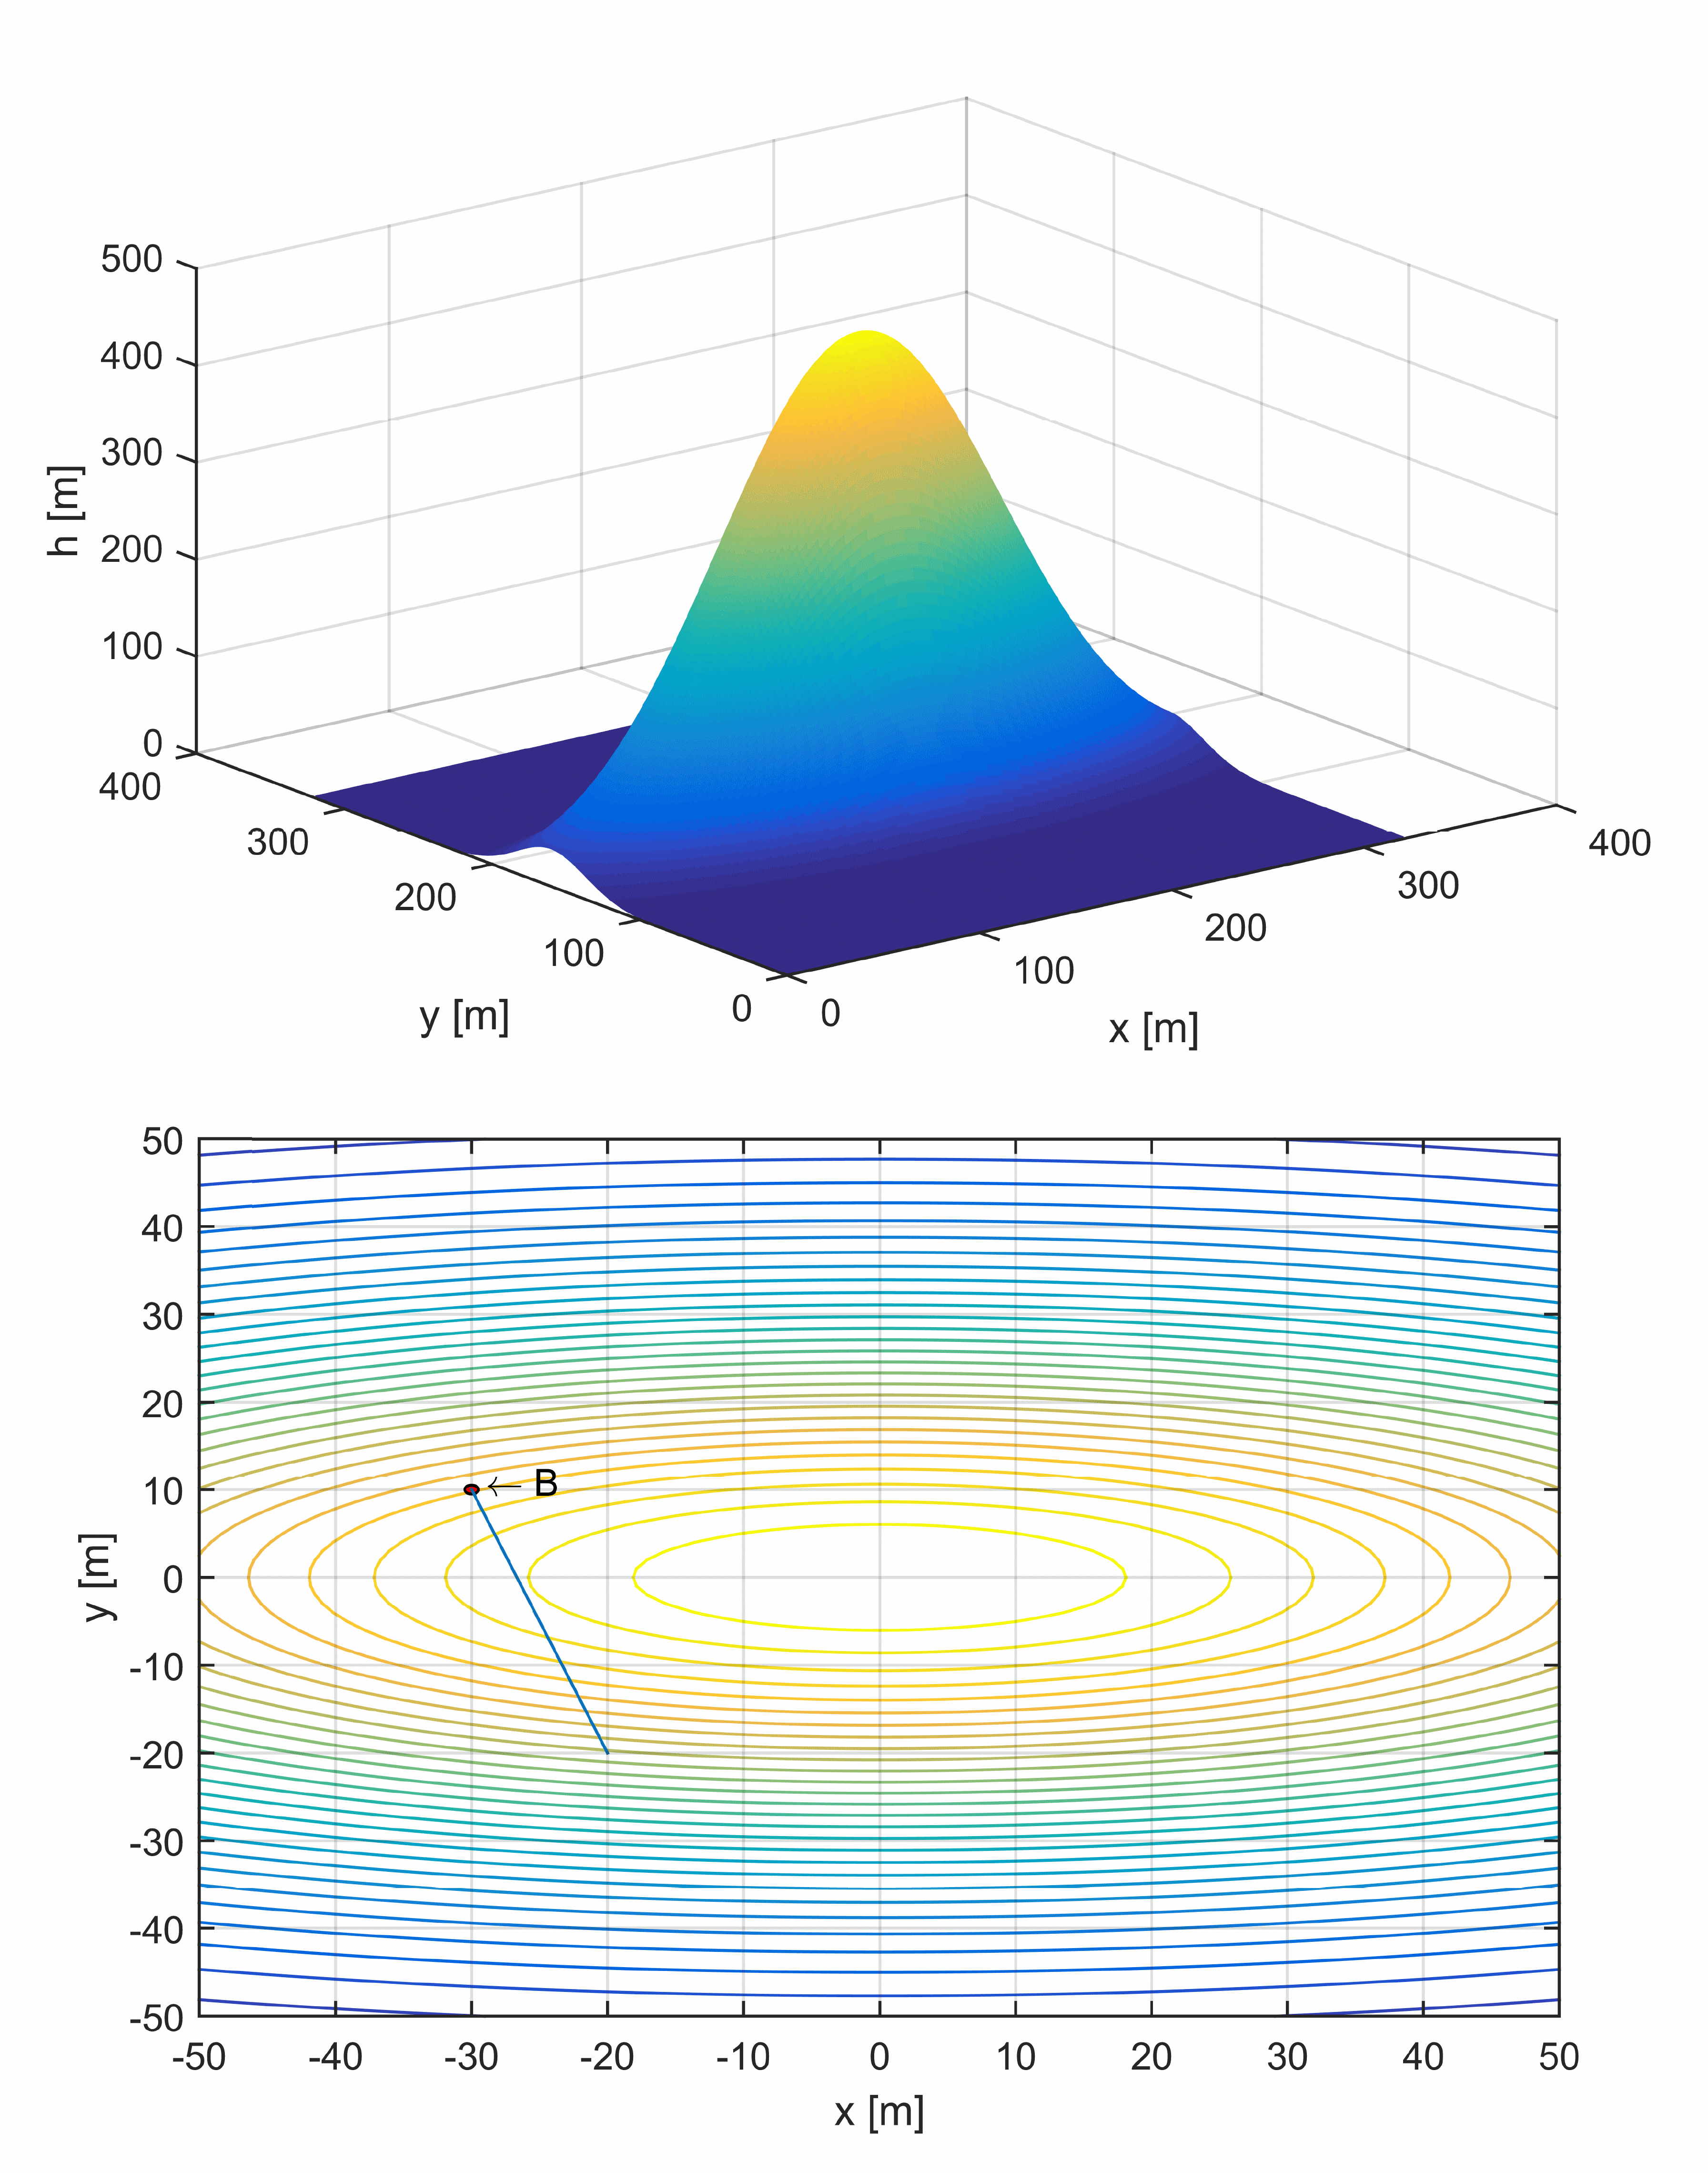
\includegraphics[width=0.9\linewidth]{fyz_fig201.png}
    \captionof{figure}{ }
    \label{fyz:fig017}
  \par}
  
  \textbf{Řešení}: Směr největšího stoupání vyjadřuje gradient skalární funkce, kterou je popsána 
  povrchová plocha kopce. Platí
  \begin{align*}
    \vec{n} &= \grad h = \left(\pder{h}{x}, \pder{h}{y}\right)   \\
            &= \frac{2A}{l_0}\exp{\left[
                 −\left(\frac{x}{l_0}\right)^2
                 −9\left(\frac{y}{l_0}\right)^2
               \right]}(x,9y) \approx (-x,-9y)
  \end{align*}
  Nepodstatné konstanty mění jen délku vektoru, nikoliv jeho směr, proto jsou v konečném  výsledku 
  vynechány. V bodě \(B\) je tedy směr největšího stoupání určen vektorem
  \begin{equation*}
   \vec{n}_B \approx (+30, –90) \approx (+10, –30) \approx (+1, –3).
  \end{equation*}
  \begin{itemize}
    \item zdroj: \librariaALDBR
    \item Matlab skript \texttt{FYZ0007.m}: 
%       \attachfile[icon=Paperclip, description=FYZ000.m]{../SRC/FYZ/matlab/FYZ000.m}
  \end{itemize}   
\end{example}